
\documentclass[a4paper,12pt]{report}% azczxc

% \documentclass{article}% use option titlepage to get the title on a page of its own.
% \usepackage{blindtext}
\usepackage{hyperref}
\usepackage{graphicx}
\graphicspath{ {./images/} }

\title{FTDI Programmer User Manual \\ $\beta$ Version}
\date{\today}
\author{Kunal Chakraborty \\kunalc@cdot.in}

\setlength{\parindent}{0pt}
\setlength{\parskip}{1em}

\begin{document}
\maketitle
\tableofcontents

%% table of content ... list of fig...


\section{Introduction}\label{intro}	% to be used with \ref{intro}



FTDI-programmer is an application written in pure python to access/program on board devices through FTDI devices 
using JTAG/SPI/I2C/GPIO interfaces. JTAG programming is done through svf file. It can be used in place of any 
external emulator. The application is built on \href{https://github.com/eblot/pyftdi}{PyFtdi driver}.



The source code is compatible with both Windows and Linux system. However this manual is written from a windows 
user's point of view.


This is a $\beta$-version and hence the application has couple of limitations as listed in section \ref{sec:limit} 

	

\section{Features}
\begin{itemize}
	\item
	On board device programming through JTAG interface. It needs svf file for JTAG programming.
	
	\item
	TI UCD device programming through I2C interface. It needs SMBUS csv file programming. This file can be
	generated by Fusion tool.
	
	\item
	SPI Flash programming.(to be implemented)
	
	\item
	On board device access thhrough SPI/I2C/GPIO interfaces. (to be implemented)

\end{itemize}	

	

\section{Limitation}\label{sec:limit}
\begin{enumerate}
	\item I2C mode
		\begin{enumerate}
			\item 
			FTDI devices does not support multimaster and clock stretching. Hence this application will not work with
			slave devices which requires clock stretching. In that case application can be run on lower frequency
			so that target device may get enough time to respond. However there is a workaround given by FTDI by 
			connecting I2C SCL to a separate gpio of FTDI device so that FTDI device can read the clock line. This 
			feature is not supported in present version FTDI-programmer.

			\item	
			Highest I2C slave address supported is 0x78. It is the limitation from pyftdi driver. No workaround is provided.
		\end{enumerate}
	
	\item	JTAG mode
		\begin{enumerate}
			\item Target device must be the only device in JTAG chain because SVF parser of FTDI-programmer does not support
			header and trailer addition. This is kept as Future Development.
			\item
			SVF file verification takes longer than expected. This is because pyftdi driver takes long time to send data to 
			application after reading from usb. This is kept as Future Development.
			\item
			Only Max-V CPLD programming is supported. If any other device is detected, FTDI-programmer will flag a warning
			with device id and exit.  
		\end{enumerate}

	\item	Others
		\begin{enumerate}
			\item 
			MS Windows detects every channel of FTDI device as a separate usb device with same VID and PID. Hence FTDI-programmer
			can access only single channel of FTDI device. So user must enable a single lib-usb driver as per FTDI channel number
			as discussed in section \ref{sec:install}
		\end{enumerate}
	\end{enumerate}	


\section{Installation}\label{sec:install}
	All the required python packages are compiled and supplied with FTDI-programmer. However it needs a low level backend driver
	libusb to talk to FTDI device. You must have admin privilege to carry out below steps.
	Step by step installation guide is given below.
	\begin{description}
		\item [1. libusb installation:]
		An easy way to install libusb backend on windows is Zadig. Download the latest version of Zadig from \url{https://zadig.akeo.ie/} %url = https://zadig.akeo.ie/
		Run zadig.exe and you should get a dialog as shown in Fig\ref{fig:zadig_main}.
			% figure -----
		
			\begin{figure}[h]
				
				\centering
				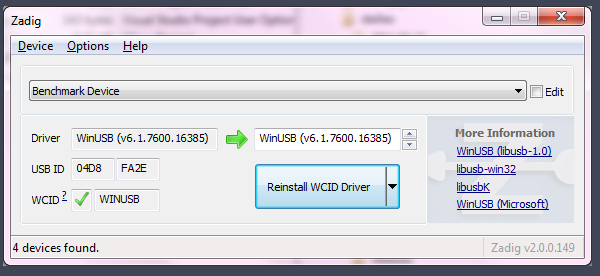
\includegraphics[scale = 0.7]{zadig_main}
				\caption{zadig main window}
				\label{fig:zadig_main}
			\end{figure}
		
		
		
		Go to Options -- List All Devices. Then select FTDI-channel0 from drop down option. Next select libusb-win32 as driver.
			% figure -----
			\begin{figure}[h]
				
				\centering
				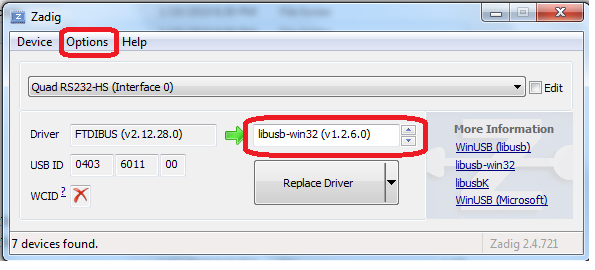
\includegraphics[scale = 0.7]{zadig_libusb}
				\caption{libusb installation}
				\label{fig:zadig_libusb}
			\end{figure}
			
		Finally, click install driver.
		Follow the same step to install driver on FTDI-channel1
		
		\item [2. Verify libusb driver:]
		Go to windows device manager. You should be able to see libusb device. Under libusb, FTDI devices
		(1 for each channel) should be shown 
		for which libusb driver is installed(refer to figure \ref{fig:device_manager}. Disable all 
		channels except one channel(the one you want to use for programming). 
		
			\begin{figure}[h]
				
				\centering
				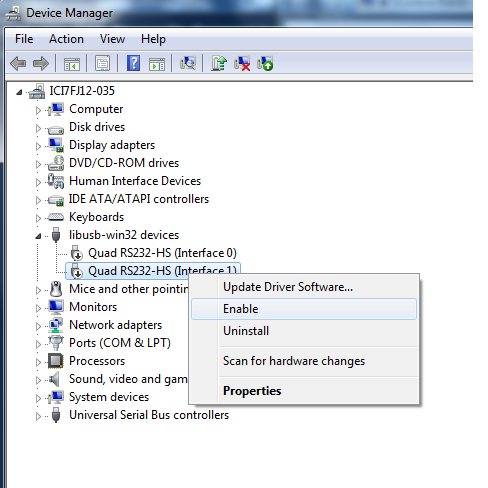
\includegraphics[scale = 0.7]{ft_channel_enable}
				\caption{Enabling FTDI channel from device manager}
				\label{fig:device_manager}
			\end{figure}
			
		
		
		\item [3. Get FTDI-programmer:]
		Download a fresh copy of FTDI-programmer from \url{https://github.com/kunalcdot/FTDI-programmer}. The application is 
		under /bin folder. Run FTDI-programmer.exe to start the application.
		
	\end{description}
	



\section{Programming Guide}\label{sec:prog_guide}
	\subsection{Programming file}
	\begin{itemize}
		\item
		For JTAG programming standard svf file needs to be used.
		
		\item
		For UCD programming, SMBUS flash script in csv format needs to be generated. The script generation procedure is
		discussed in detail in section \ref{sec:script}
		
		
	\end{itemize}	
	
	
	\subsection{SMBUS script generation}\label{sec:script}
	UCD devices run on SMBUS protocol. FTDI-programmer sends SMBUS commands towards UCD device for programming. TI Fusion
	tool can be used to generate SMBUS flash script. Note that flash script can only be generated in online mode. Also note
	that the UCD device used to generate flash script should have the same firmware as target device. This will also be verified by
	FTDI-programmer.
	
	Open Fusion GUI tool in online mode. Then go to File -- Export option. Under export option select \textbf{'Data Flash Script'}.
	Select below mentioned options in the script settings:
	\begin{itemize}
		\item
		Script Style: SMBUS
		\item
		Add PEC byte
		\item
		File format: CSV
		\item
		Hex format: 0xAABB
		\item
		Comment Style: 'Comment'
		\item
		Multiple byte: Compact
		\item
		Read verification: As per your choice
	\end{itemize}	

	A screenshot of script settings is shown in figure \ref{fig:smbus_script}. Export the file with .csv extension.
	
	
	
		\begin{figure}[p]
				
				\centering
				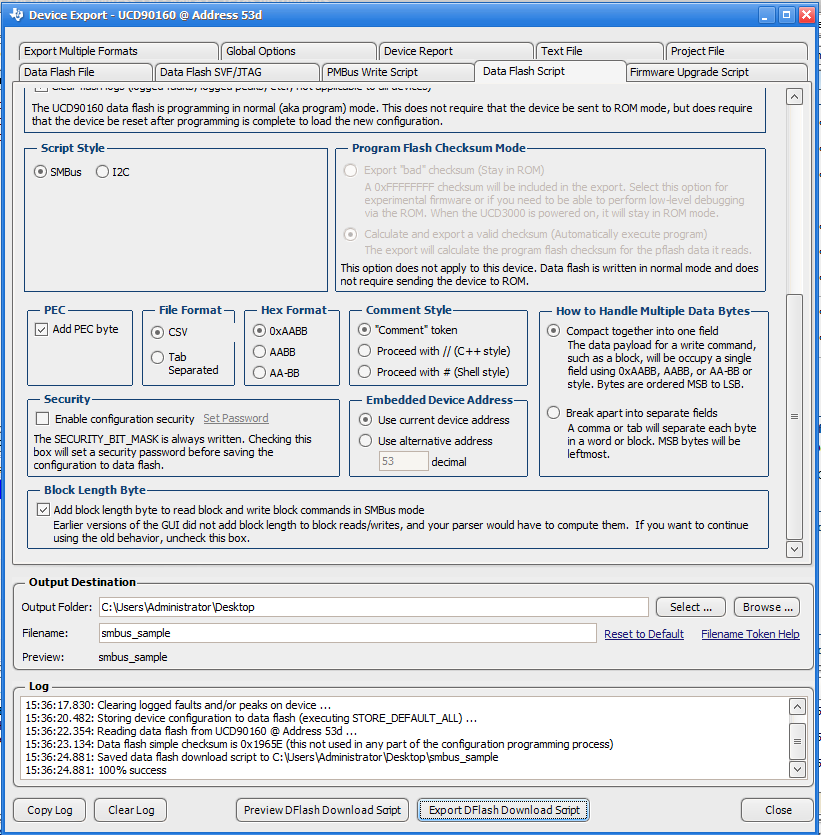
\includegraphics[scale = 0.7]{smbus_flash_script_generation}
				\caption{SMBUS Flash Script for UCD device}
				\label{fig:smbus_script}
			\end{figure}
	
	
	
	
	
	\subsection{FTDI Channel selection}
	Due to limitation from MS Windows, PC running FTDI-programmer must have only one channel active. Libusb driver 
	can be installed on multiple channels. However ensure that all the channels except the desired channel are disabled.
	This can be done in windows device manager utility. Refer to Figure \ref{fig:device_manager}. The user must have
	administrator privilege. 
	
	
	\subsection{Run FTDI-programmer}
	Download a fresh copy of FTDI-programmer from \url{https://github.com/kunalcdot/FTDI-programmer}. The application is 
	under /bin folder. Run FTDI-programmer.exe to start the application. Ensure all supporting files(dll and windows api)
	are present in same directory.
	
	There are 2 programming modes: JTAG(standard svf programming) and I2C(customized UCD device programming). Each mode 
	supports default as well as advance settings. Most of the time default setting is the desired one. In advance mode, you
	can change programming frequency and frequency optimization. 
	
	For JTAG default frequency is 3MHz. FTDI-programmer ignores svf file frequency command. In case of I2C default frequency
	is 5KHz. As FTDI device does not support clock stretching, default frequency is kept low to communicate with UCD device.
	
	Next browse the file to be progrmmed and programming will be started.  	
		
		
		
\section{Future Development}
\begin{enumerate}
	\item 
	All programming file parser to be updated with 'regular expression' module. It should support all svf standard command.
	
	\item 
	JTAG read time needs to be reduced.
	
	\item 
	SPI Flash Programming option to be developed
	
	\item 
	An utility needs to be provided to read/write on board devices through I2C/SPI/GPIO etc

\end{enumerate}

\section{Troubleshooting}
Ensure only one FTDI device is connected and single ftdi channel is enabled. Refer to section \ref{sec:install} for more details.

Error: No ftdi device	-- Ensure pc is connected to FTDI device and the device is out of reset

% Error: No backend available : ensure  'libusb0.dll' and 'libusb0_x86.dll' files are present in /bin folder. 

Error: Unknown device detected(In jtag mode): Ensure board is powered up and there is only one device(MAX-V) in JTAG chain.

Error: File not found: Ensure there is no white space in your file path.



\end{document}